\subsection{Princípios SOLID}

    \par Os princípios SOLID, um acrônimo popularizado por Michael Feathers com base nos trabalhos de Robert C. Martin, representam cinco diretrizes cruciais para o design de software orientado a objetos. Estes princípios foram concebidos para auxiliar os desenvolvedores a construir sistemas que sejam mais fáceis de entender, manter e evoluir, aplicando-se a classes em qualquer camada da aplicação para se alcançar um melhor design, o que, por sua vez, contribui para uma base de código flexível e de fácil manutenção \cite{livro:joshi:2016}.

    \par A adesão a estes cinco preceitos — Princípio da Responsabilidade Única (SRP), Princípio Aberto/Fechado (OCP), Princípio da Substituição de Liskov (LSP), Princípio da Segregação de Interface (ISP) e Princípio da Inversão de Dependência (DIP) — é fundamental para o desenvolvimento de software de alta qualidade. Eles oferecem um vocabulário comum e um conjunto de heurísticas para a discussão e avaliação da arquitetura de software, direcionando as práticas de desenvolvimento para a minimização de dependências e o aprimoramento da coesão do código \cite{artigo:ramachandrappa:2024}.
    
    \par Cada princípio é descrito abaixo, com sua aplicação e exemplos práticos.

%
%
% SRP
%
%
    
\subsection{Princípio da Responsabilidade Única (Single Responsibility Principle - SRP)}
    
    \par O Princípio da Responsabilidade Única (SRP) preconiza que um módulo, ou mais comumente uma classe, deve ter uma, e apenas uma, razão para mudar, o que implica ser responsável por um único ator ou aspecto da funcionalidade do sistema. Este princípio está intimamente ligado ao conceito de coesão, onde um módulo coeso agrupa funcionalidades que servem a um único propósito bem definido. O objetivo é garantir que cada classe realize uma tarefa específica, simplificando sua compreensão e manutenção \cite{livro:martin:cleanarch}.

    \par A aplicação do SRP é vital, pois assegura que cada classe permaneça dedicada a uma tarefa específica, o que, por sua vez, simplifica seu entendimento, manutenção e potencial de expansão. Quando as classes seguem o SRP, elas se tornam mais diretas para refatorar, testar e estender, e modificações são menos propensas a afetar outras partes do sistema, minimizando o risco de introduzir erros. Isso é um contraste com classes que acumulam múltiplas responsabilidades, as quais se tornam complexas e frágeis \cite{artigo:ramachandrappa:2024}.

    \par Segue um exemplo prático de violação do SRP, conforme pode ser visualizado na Figura~\ref{fig:figura_srp_bad} que demonstra a situação ANTES da aplicação do princípio:
        
    \begin{figure}[H]
        \centering
        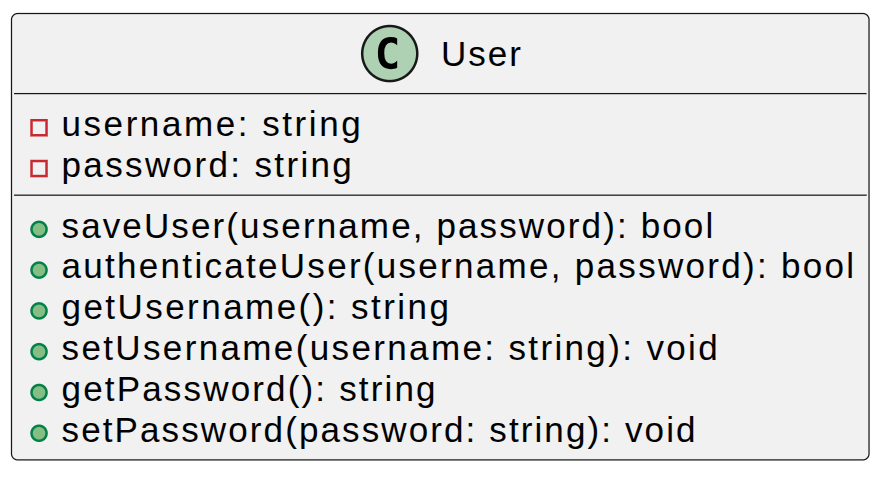
\includegraphics[width=0.8\textwidth]{figuras/solid/srp_bad.png}
        \caption{Violação do SRP.}
        \label{fig:figura_srp_bad}
        \newcommand{\minhafonte}{Fonte: Adaptado de \cite{artigo:ramachandrappa:2024}.}
        \minhafonte
    \end{figure}

    \par Nesse exemplo trazido por \cite{artigo:ramachandrappa:2024} a classe User que lida tanto com a gestão dos dados do usuário (como nome e senha) quanto com a lógica de autenticação desse usuário, como no método AuthenticateUser. 
    
    \par A Figura~\ref{fig:figura_srp_good} ilustra a situação DEPOIS da refatoração para fazer uso do SRP:

    \begin{figure}[H]
        \centering
        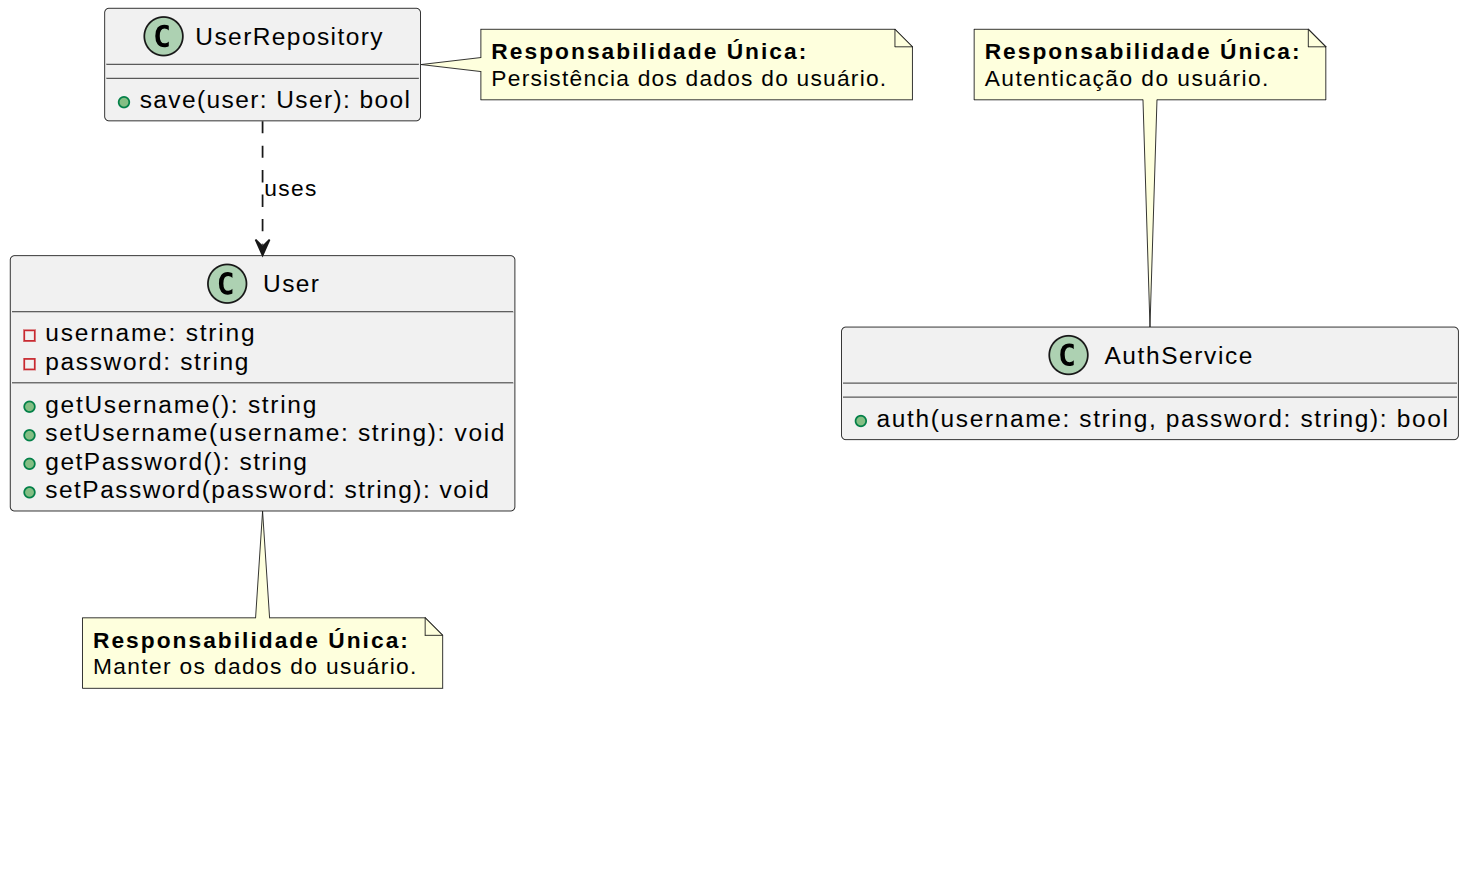
\includegraphics[width=0.9\textwidth]{figuras/solid/srp_good.png}
        \caption{Aplicação do SRP.}
        \label{fig:figura_srp_good}
        \newcommand{\minhafonte}{Fonte: Adaptado de \cite{artigo:ramachandrappa:2024}.}
        \minhafonte
    \end{figure}

    \par Na Figura~\ref{fig:figura_srp_good} a classe User mantêm apenas os dados, a classe UserRepository controla a persistência e AuthService gerenciaria a autenticação, assim demonstrando o uso da SRP, onde cada classe tem sua própria responsabilidade \cite{artigo:ramachandrappa:2024}.

        

%
%
% OPC
%
%
\subsection{Princípio Aberto/Fechado (Open/Closed Principle - OCP)}

    \par O OCP determina que classes devem ser abertas para extensão, mas fechadas para modificação, assim permitindo a adição de funcionalidades sem alterar o código existente \cite{livro:martin:cleanarch}. Na Arquitetura Limpa, o OCP é implementado por meio de interfaces e herança, especialmente em adaptadores, para suportar novas integrações \cite{livro:martin:cleanarch}. 

    \par O Princípio Aberto/Fechado (OCP), conforme articulado por Bertrand Meyer, estabelece que entidades de software, como classes, módulos ou funções, devem ser abertas para extensão, mas fechadas para modificação. Isso significa que o comportamento de um sistema deve poder ser estendido através da adição de novo código, em vez de alterar código existente que já foi testado e está em funcionamento. Este princípio visa proteger o código existente de regressões e reduzir a necessidade de retestes extensivos \cite{livro:martin:cleanarch}.

    \par Seguir o OCP é crucial para manter a estabilidade do software à medida que ele evolui, permitindo que novas funcionalidades sejam integradas sem comprometer as existentes. Ao aderir ao OCP, os desenvolvedores podem adicionar novas funcionalidades sem alterar o código base existente, o que minimiza o risco de introduzir novos bugs. Este princípio é crucial para criar sistemas que podem crescer e se adaptar ao longo do tempo com menor esforço de manutenção \cite{artigo:ramachandrappa:2024}.


    \par Considere uma classe DiscountCalculator que calcula descontos com base em diferentes tipos de cliente através de múltiplas declarações if-else if, como pode ser visualizado no diagrama ANTES da aplicação do OCP:

     \begin{figure}[H]
        \centering
        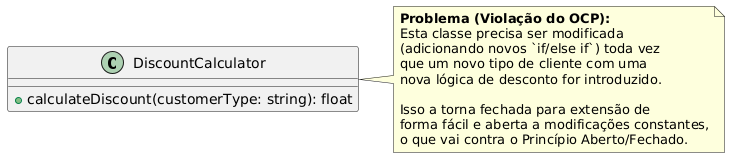
\includegraphics[width=0.8\textwidth]{figuras/solid/ocp_bad.png}
        \caption{Violação da OCP.}
        \label{fig:figura_ocp_bad}
        \newcommand{\minhafonte}{Fonte: Adaptado de \cite{artigo:ramachandrappa:2024}.}
        \minhafonte
    \end{figure}
        
    Para aplicar o OCP, como demonstrado no diagrama DEPOIS da aplicação do OCP:

     \begin{figure}[H]
        \centering
        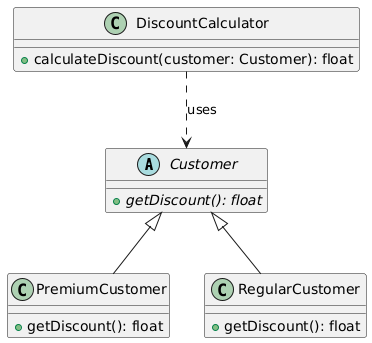
\includegraphics[width=0.5\textwidth]{figuras/solid/ocp_good.png}
        \caption{Aplicação da OCP.}
        \label{fig:figura_ocp_good}
        \newcommand{\minhafonte}{Fonte: Adaptado de \cite{artigo:ramachandrappa:2024}.}
        \minhafonte
    \end{figure}

    pode-se usar polimorfismo: uma classe abstrata Customer com um método abstrato GetDiscount(). As classes RegularCustomer e PremiumCustomer herdariam de Customer e implementariam GetDiscount(). Assim, o DiscountCalculator usaria o método GetDiscount() do objeto Customer passado, permitindo a adição de novos tipos de clientes criando novas subclasses de Customer sem alterar o DiscountCalculator \cite{artigo:ramachandrappa:2024}.



%
%
% LSP
%
%
\subsection{Princípio da Substituição de Liskov (Liskov Substitution Principle - LSP)}

    \par O Princípio da Substituição de Liskov (LSP), formulado por Barbara Liskov, dita que instâncias de uma classe pai devem ser substituíveis por instâncias de uma classe derivada sem alterar a corretude ou o comportamento esperado do programa. Este princípio é crucial para guiar o uso da herança de forma a manter a integridade e a previsibilidade do sistema. Essencialmente, uma subclasse deve poder ser utilizada em qualquer lugar onde sua superclasse é esperada, sem causar efeitos colaterais indesejados \cite{livro:martin:cleanarch}.

    \par Aderir ao LSP é fundamental para o uso correto do polimorfismo e da herança, resultando em código mais confiável e de fácil manutenção, especialmente em sistemas grandes onde o polimorfismo é intensamente utilizado. Quando o LSP é respeitado, as hierarquias de classes são mais robustas, e a capacidade de substituição garante que o sistema se comporte de maneira consistente, independentemente da implementação específica da subclasse utilizada \cite{livro:joshi:2016}.
    
    \par Um exemplo clássico de violação do LSP, que pode ser detalhado no diagrama ANTES da aplicação do LSP:
    
    \begin{figure}[H]
        \centering
        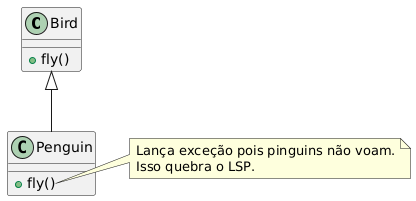
\includegraphics[width=0.7\textwidth]{figuras/solid/lsp_bad.png}
        \caption{Violação da LSP.}
        \label{fig:solid/lsp_bad}
        \newcommand{\minhafonte}{Fonte: Adaptado de \cite{artigo:ramachandrappa:2024}.}
        \minhafonte
    \end{figure}
    
    ocorre com as classes Rectangle e Square, ou Bird e Penguin. No caso Bird/Penguin, se Penguin herda de Bird e o método Fly() em Bird implica a capacidade de voar, a implementação de Fly() em Penguin (que não voa) lançando uma exceção violaria o LSP. Uma solução, apresentada no diagrama DEPOIS da refatoração:
    
    \begin{figure}[H]
        \centering
        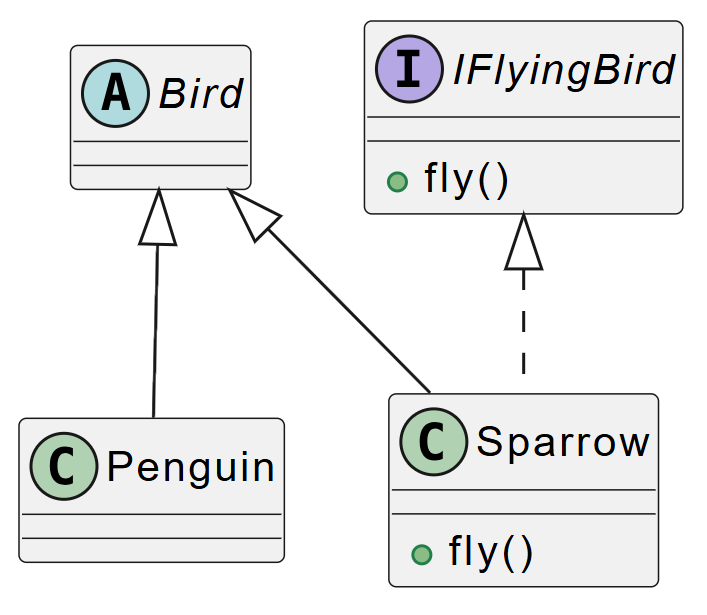
\includegraphics[width=0.5\textwidth]{figuras/solid/lsp_good.png}
        \caption{Aplicação da LSP.}
        \label{fig:figura_lsp_good}
        \newcommand{\minhafonte}{Fonte: Adaptado de \cite{artigo:ramachandrappa:2024}.}
        \minhafonte
    \end{figure}
    
    poderia envolver hierarquias mais adequadas ou interfaces específicas para as capacidades, como uma interface IFlyingBird não implementada por Penguin \cite{artigo:ramachandrappa:2024}.


%
%
% ISP
%
%
\subsection{Princípio da Segregação de Interface (Interface Segregation Principle - ISP)}
    
    \par O Princípio da Segregação de Interface (ISP) orienta que os clientes de uma classe não devem ser forçados a depender de métodos que não utilizam. Este princípio promove a criação de interfaces menores, coesas e específicas para as necessidades de cada cliente, em detrimento de interfaces grandes e genéricas que tentam abranger múltiplas funcionalidades. O objetivo é evitar que classes implementem métodos desnecessários, o que pode levar a um acoplamento indesejado \cite{livro:martin:cleanarch}.

    \par A aplicação do ISP é importante para promover o desacoplamento, assegurando que as classes dependam apenas das interfaces que são estritamente relevantes para elas. Isso não apenas reduz o impacto de futuras alterações – já que uma mudança em uma interface específica afeta apenas os clientes que a utilizam – mas também torna a base de código mais flexível, modular e fácil de testar. Interfaces menores são mais fáceis de entender e implementar corretamente \cite{artigo:ramachandrappa:2024}.
    
    \par Um exemplo de violação do ISP, que pode ser visualizado na Figura~\ref{fig:figura_isp_bad}:
    
     \begin{figure}[H]
        \centering
        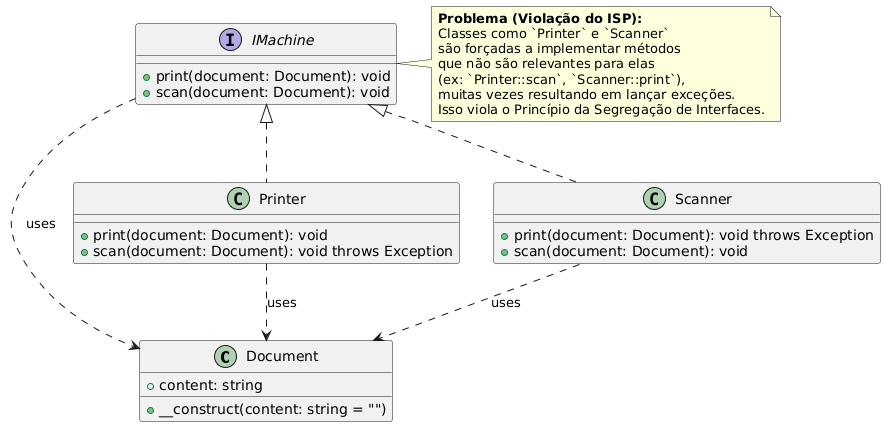
\includegraphics[width=0.9\textwidth]{figuras/solid/isp_bad.png}
        \caption{Violação da ISP.}
        \label{fig:figura_isp_bad}
        \newcommand{\minhafonte}{Fonte: Adaptado de \cite{artigo:ramachandrappa:2024}.}
        \minhafonte
    \end{figure}
    
    é uma interface IMachine que declara métodos como Print(Document document) e Scan(Document document). Uma classe Printer que implementa IMachine seria forçada a implementar Scan(). Para aderir ao ISP, como mostrado no diagrama das interfaces segregadas:
    
    \begin{figure}[H]
        \centering
        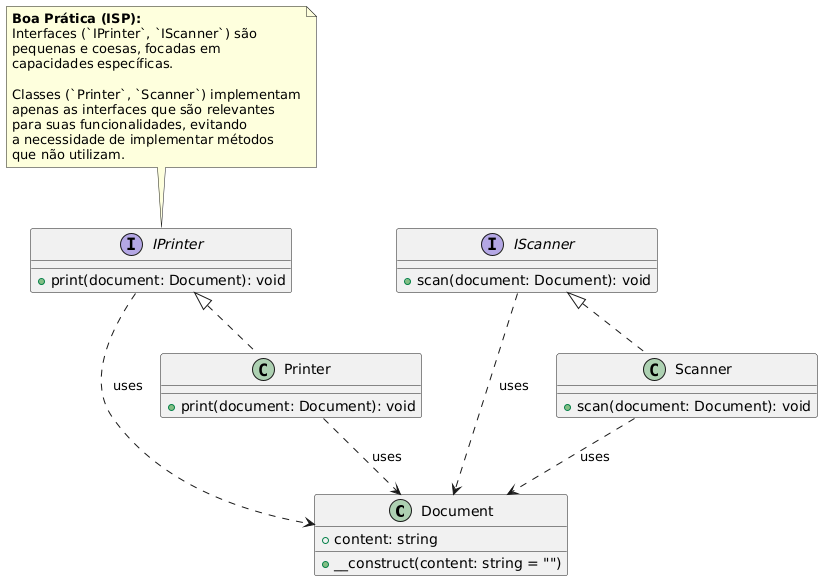
\includegraphics[width=0.9\textwidth]{figuras/solid/isp_good.png}
        \caption{Aplicação da ISP.}
        \label{fig:figura_isp_good}
        \newcommand{\minhafonte}{Fonte: Adaptado de \cite{artigo:ramachandrappa:2024}.}
        \minhafonte
    \end{figure}
    
    IMachine seria dividida em interfaces mais granulares, como IPrinter e IScanner, permitindo que Printer implemente apenas IPrinter \cite{artigo:ramachandrappa:2024}.
        
\subsection{Princípio da Inversão de Dependência (Dependency Inversion Principle - DIP)}
    
    \par O Princípio da Inversão de Dependência (DIP) estabelece que módulos de alto nível não devem depender de módulos de baixo nível; ambos devem depender de abstrações. Adicionalmente, as abstrações não devem depender de detalhes concretos, mas sim os detalhes é que devem depender das abstrações. Isso significa que as classes que contêm a lógica de negócios principal (alto nível) não devem ser diretamente acopladas a classes que lidam com detalhes de infraestrutura (baixo nível) \cite{livro:martin:cleanarch}.

    \par Este princípio é crucial para criar sistemas desacoplados e flexíveis, pois promove a dependência de interfaces ou classes abstratas em vez de implementações concretas. Isso permite que as implementações de baixo nível possam ser alteradas ou substituídas sem impactar os módulos de alto nível, desde que o contrato definido pela abstração seja mantido. Tal desacoplamento também facilita os testes, permitindo a substituição de dependências reais por dublês de teste \cite{livro:joshi:2016}

    Considere o exemplo no diagrama na Figura~\ref{fig:figura_dip_bad} que ilustra a dependência concreta:

    \begin{figure}[H]
        \centering
        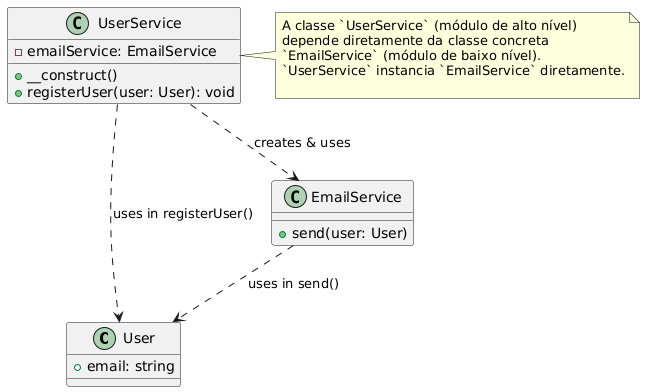
\includegraphics[width=0.9\textwidth]{figuras/solid/dip_bad.png}
        \caption{Violação da DIP.}
        \label{fig:figura_dip_bad}
        \newcommand{\minhafonte}{Fonte: Adaptado de \cite{artigo:ramachandrappa:2024}.}
        \minhafonte
    \end{figure}

    onde uma classe UserService (alto nível) que depende diretamente de uma classe concreta EmailService (baixo nível) está fortemente acoplada. Para aplicar o DIP, como ilustrado no diagrama que demonstra a inversão de dependência:

    
    \begin{figure}[H]
        \centering
        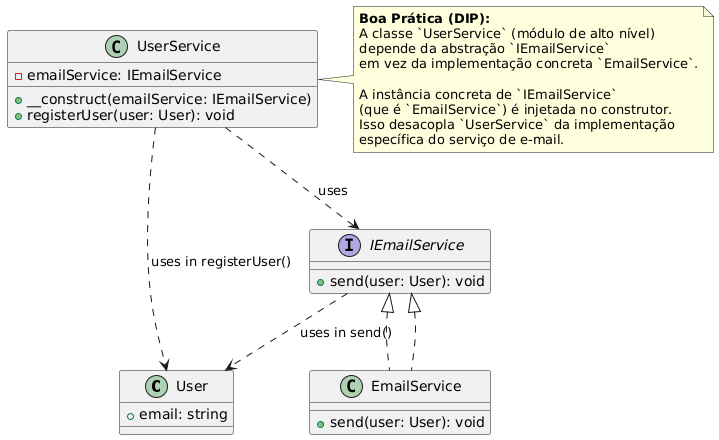
\includegraphics[width=0.9\textwidth]{figuras/solid/dip_good.png}
        \caption{Aplicação da DIP.}
        \label{fig:figura_dip_good}
        \newcommand{\minhafonte}{Fonte: Adaptado de \cite{artigo:ramachandrappa:2024}.}
        \minhafonte
    \end{figure}
    
    \par Nesse cado seria criada uma interface IEmailService. UserService dependeria de IEmailService (frequentemente via injeção de dependência), e EmailService implementaria IEmailService. Isso inverte a direção da dependência \cite{artigo:ramachandrappa:2024}.